\newpage

\section{Dependence Analysis}



\subsection{Dependence in Loops}

If there are no dependences in a loop, we can parallelize it because none of the 
iterations interfere with each other. Loop dependence is also useful in other loop optimizations, such
as loop interchange, loop fusion, etc.

In this section, we should answer the following two questions:

\begin{itemize}
\item How do we represent dependences in loops?
\item How do we determine if there are dependences?
\end{itemize}    


\subsubsection{Representing dependences}

Iteration space graphs is a good start. Here we give steps for creating 
iteration space graphs:

\begin{itemize}
    \item Step 1: Create nodes, 1 for each iteration
    \item Step 2: Determine which array elements are read and
    written in each iteration
    \item Step 3: Draw arrows to represent dependences
\end{itemize}    
    

\begin{figure}[H]
    \centering
    \begin{subfigure}{0.6\textwidth}
    \centering
        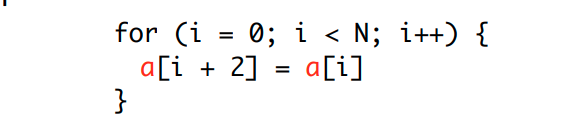
\includegraphics[width=\textwidth]{p253.png}
        \caption{Source code.}
        \label{fig:p253}
    \end{subfigure}
    \begin{subfigure}{0.6\textwidth}
    \centering
        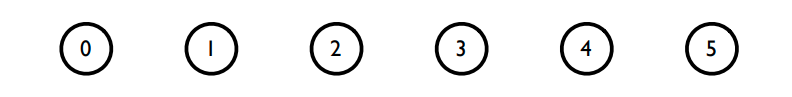
\includegraphics[width=\textwidth]{p250.png}
        \caption{Step 1: Create nodes, 1 for each iteration}
        \label{fig:p250}
    \end{subfigure}
    \begin{subfigure}{0.6\textwidth}
        \centering
            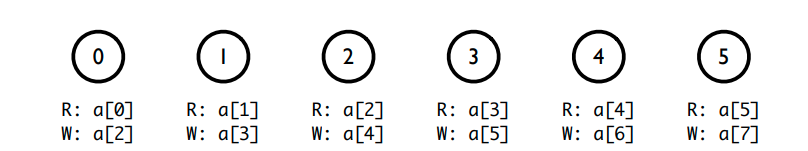
\includegraphics[width=\textwidth]{p251.png}
            \caption{Step 2: Determine which array elements are read and
            written in each iteration}
            \label{fig:p251}
        \end{subfigure}
    \begin{subfigure}{0.6\textwidth}
            \centering
                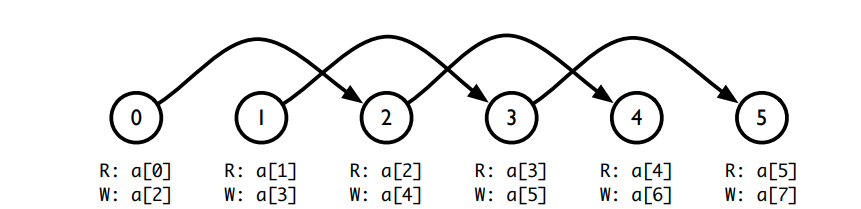
\includegraphics[width=\textwidth]{p252.png}
                \caption{Step 3: Draw arrows to represent dependences}
                \label{fig:p252}
    \end{subfigure}    
    \caption{A 1-D exmaple to illustrate Iteration space graphs.}
       \label{fig:p253}
\end{figure}



\begin{figure}[H]
    \centering
    \begin{subfigure}{0.5\textwidth}
    \centering
        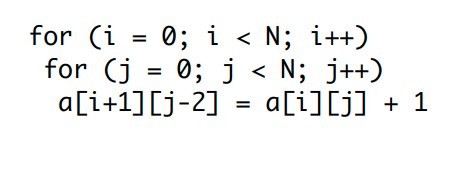
\includegraphics[width=\textwidth]{p255.png}
        \caption{Source code.}
        \label{fig:p255}
    \end{subfigure}
    \begin{subfigure}{0.5\textwidth}
    \centering
        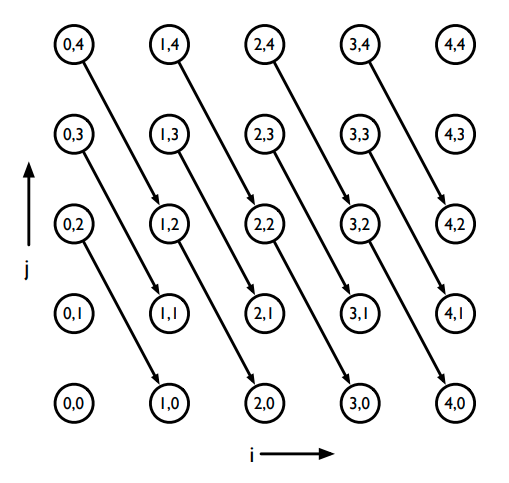
\includegraphics[width=\textwidth]{p254.png}
        \caption{Iteration space graphs for the source code.}
        \label{fig:p254}
    \end{subfigure}
  
    \caption{A 2-D exmaple to illustrate Iteration space graphs.}
       \label{fig:p254-5}
\end{figure}


But there is a crucial problem faced by iteration space graph: 
Iteration space graphs are potentially infinite representations!

Compiler researchers have devised compressed representations of dependences, such 
as distance vectors and direction vectors.

\subsubsection{Distance vector}

Distance vectors captures the “shape” of dependences,
but not the particular source and sink. Represent each dependence arrow in an iteration space
graph as a vector.

Distance vectors for Figure \ref{fig:p252} is $ (2) $. 
Distance vectors for Figure \ref{fig:p254} is $ (1,-2) $.


A more complex example is shown in \label{fig:p256-7}.
There are 2 distance vectors : $(1,-2), (2,0)$.




\begin{figure}[H]
    \centering
    \begin{subfigure}{0.5\textwidth}
    \centering
        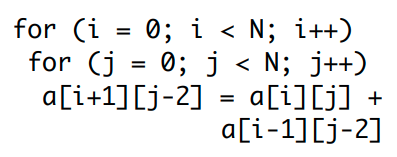
\includegraphics[width=\textwidth]{p256.png}
        \caption{Source code.}
        \label{fig:p256}
    \end{subfigure}
    \begin{subfigure}{0.5\textwidth}
    \centering
        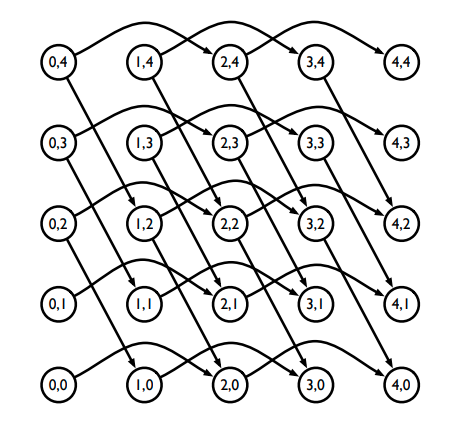
\includegraphics[width=\textwidth]{p257.png}
        \caption{Iteration space graphs for the source code.}
        \label{fig:p257}
    \end{subfigure}
  
    \caption{A 2-D exmaple to illustrate Iteration space graphs.}
       \label{fig:p256-7}
\end{figure}


But distance vectors can't always summarize as easily. Consider the example in
\ref{fig:p258}, distance vectors for this code are $(1), (2), (3), (4) ...$



\begin{figure}[H]
    \centering
    \begin{subfigure}{0.5\textwidth}
    \centering
        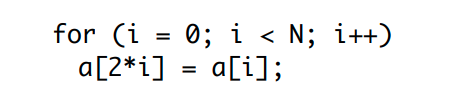
\includegraphics[width=\textwidth]{p258.png}
        \caption{Source code.}
        \label{fig:p258}
    \end{subfigure}
    \begin{subfigure}{0.7\textwidth}
    \centering
        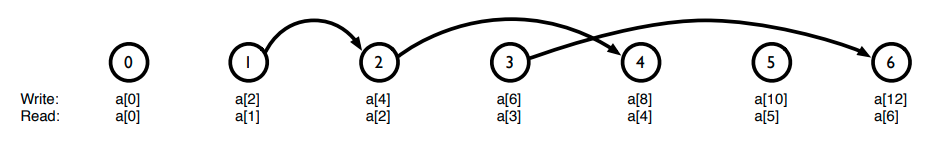
\includegraphics[width=\textwidth]{p259.png}
        \caption{Iteration space graphs for the source code.}
        \label{fig:p259}
    \end{subfigure}
  
    \caption{A 2-D exmaple to illustrate Iteration space graphs.}
       \label{fig:p258-9}
\end{figure}

From distance vector, we have information about the length of each vector,
but not about the source of each vector. What happens if we try to reconstruct the iteration space graph?



\begin{figure}[H]
    \centering
    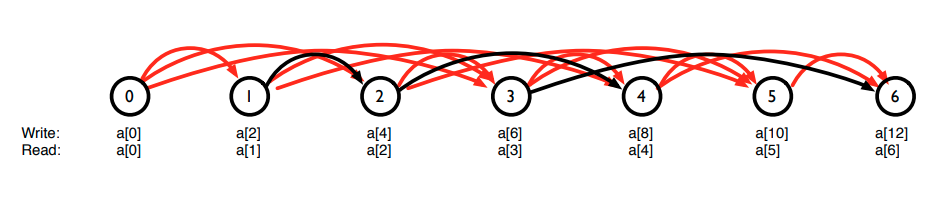
\includegraphics[width=0.8\textwidth]{p260.png}
    \caption{reconstruct the iteration
    space graph from distance vector for \ref{fig:p258}}
    \label{fig:p260}
\end{figure}


\subsection{Direction vectors}

The whole point of distance vectors is that we want to be able to
succinctly capture the dependences in a loop nest and summarize distance vectors, and save only the direction the
dependence was in.


For example, distance vector $(2,-1)$, the corresponding direction vector is $(+,-)$.
Also, distance vector $(0,1)$, the corresponding direction vector is $(0,+)$.

Direction vectors lose a lot of information, but do capture
some useful information, such as whether there is a dependence (anything other than a
$0$ means there is a dependence). 
Many times, the only information we need to determine if
an optimization (e.g. loop paralelization, loop iterchange) is legal is captured by direction vectors. 



If there is a non-zero entry for a loop dimension, that
means that there is a loop carried dependence over that
dimension. If an entry is zero, then that loop can be parallelized!





\subsubsection{Loop-carried dependence}

Loop carried dependence is a dependence that crosses loop iterations.

If there is a  loop carried dependence, then that loop cannot
be parallelized. 


\subsection{Data Dependence Tests}


\subsubsection{GCD}



\begin{figure}[H]
    \centering
    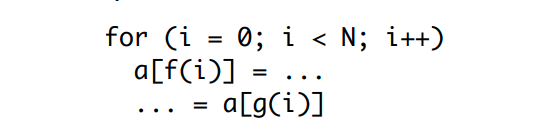
\includegraphics[width=0.6\textwidth]{p261.png}
    \caption{}
    \label{fig:p261}
\end{figure}

Consider the loop nest in \ref{fig:p261} , A dependence exists if there exist an integer $i$ and an $i^\prime$ such
that:
\begin{itemize}
    \item  $f(i) = g(i^\prime)$
    \item  $0 \leq i, i^\prime < N$
    \item  If $i < i^\prime$, write happens before read (flow dependence)
    \item  If $i > i^\prime$, write happens after read (anti dependence)
\end{itemize}




An equation $a_1 \times i + a_2 \times i^\prime = a_3$ has a solution iff $gcd(a_1, a_2)$
evenly divides $a_3$

For example,
\begin{itemize}
    \item $15 \times i + 6 \times j - 9 \times k = 12$ has a solution (gcd = 3)
    \item $2 \times i + 7 \times j = 3$ has a solution (gcd = 1)
    \item $9 \times i + 6 \times j = 10$ has no solution (gcd = 3)
\end{itemize}



Unfortunately, most loops have gcd(a, b) = 1, which divides
everything. Also, If $f(i) = g(i^\prime)$, there might be a dependence, 
but might not.
